%% main.tex
%% Distributed with umalayathesis v1.5 (28 October 2018)
\documentclass[english,singlespacedlisttitles]{umalayathesis}
%% Document class options
%% -----------------------
%% english (default): English thesis
%%
%% bahasam : Malay thesis
%%
%% apacite (default): Loads the apacite package, which implements the APA
%%    citation and referencing styles strictly, including expansion of
%%    of 3–5 authors on first citation.
%%
%% newapa: Loads the natbib and apalike package for a APA-like reference list
%%    but *does not fully implement* all APA citation styles. In particular,
%%    this option will not expand references with 3–5 authors on first citation.
%%    NOT RECOMMENDED UNLESS EXPLICITLY REQUESTED BY EXAMINER.
%%
%% custombib: Does not pre-load any bibliography style; you will need to
%%    specify \bibliographystyle, \bibliographystyleown etc yourself.
%%
%% appendixhead: Add "APPENDICES" before the Appendix A title
%%
%% altcaption: Caption in smaller fonts; only Figure X, Table Y bold.
%%
%% singlespacedlisttitles: Long titles in the ToC, LoT, LoF, LoA are single-spaced.
%%
%% listpageheader: If your faculty requires a "header row" at the top of
%%    the List of Figures/Tables. You can re-define \lofpageheader and
%%    \lotpageheader if necessary, e.g.
%%           \renewcommand{\lofpageheader}{\hfill Page}
%%
%% boldfrontmattertoc: If your faculty wants front matter "chapters" to be
%%    bold in the ToC
%%
%% boldbackmattertoc: If the backmatter "chapters" are to be bolded as well
%%
%% uppercasetoc: If all "chapter" level headings must be upper-cased in the ToC

\usepackage{lipsum}
\usepackage[utf8]{inputenc}
\usepackage[T1]{fontenc}
\usepackage{microtype}
\usepackage{graphicx}
\usepackage{caption}
\usepackage[dvipsnames,x11names]{xcolor}
\usepackage{listings}
\usepackage{glossaries}

% For the process flow diagram in chapter 3
\usepackage{tikz}
\tikzstyle{block} = [rectangle, draw, fill=blue!20, text width=10em, text centered, rounded corners, minimum height=4em]
\tikzstyle{line} = [draw, -latex]

% Useful for including code listings
\usepackage{listings}
\lstset{language=[LaTeX]TeX,columns=fullflexible,
        basicstyle=\ttfamily\SingleSpacing,
        texcsstyle=*\bfseries\color{NavyBlue},
        commentstyle=\itshape\color{PaleVioletRed4},
        frame=single,framesep=6pt,
        framexleftmargin=6pt,framexrightmargin=6pt,
        xleftmargin=12pt,xrightmargin=12pt,
        breaklines=true,breakatwhitespace=true,
        aboveskip=-1.5\onelineskip
}

% Useful for multi-page pages. Either longtable or supertabular is fine; choose any one that you're comfortable with
\usepackage{longtable}
% \usepackage{supertabular}


\author{Ng Kang Wei}
\title{Text Classification with Dimension Reduction on News Articles}

%% If \othertitle is given, then the second abstract will display it
%% (i.e. if your thesis is "english" then this is printed on top of the Malay abstract
%% and if your thesis is "bahasam" then this is printed on top of the English abstract)
%% If no \othertitle is given then the second abstract will not have any translated thesis title
%\othertitle{Tajuk dalam Bahasa Lain untuk Abstrak Kedua}

\faculty{Department of Computer Science and Information Technology}
\submissionyear{2019}
\degree{Master of Data Science}

% load acronym definitions from separate file
\makeglossaries
\loadglsentries[acronym]{myacronyms}


\begin{document}
\frontmatter

%% Choose only ONE from the following to get the
%% correct statement on the title page
\makecoverandtitlepage{\mastercoursework}
% \makecoverandtitlepage{\mastermixedmode}
% \makecoverandtitlepage{\masterresearch}
% \makecoverandtitlepage{\doctoralcoursework}
% \makecoverandtitlepage{\doctoralresearch}
% \makecoverandtitlepage{\doctoralmixedmode}

\declarationpage
\abstractfromfile{abstract}
%\msabstractfromfile{abstractms}
\acknowledgements{
	I would like to take this opportunity to appreciate the helps and guidance given freely by my supervisor, Dr Hoo. Without his guidance and encouragement, this study would not has seen the light of day.
	
	I am thankful and indebted to the lecturers who persevered and pour their hearts out to educate fellow students like me. It is through their hardwork and sacrifices that I have gain knowledges that are crucial to this work.
	
	I am also grateful to my fellow friends who are by my side as we work on our own projects. It is comforting to have someone working by your side towards the same goal.
}

{\clearpage\singlespacing
\tableofcontents\clearpage
\listoffigures\clearpage
\listoftables\clearpage
\listofacronyms\clearpage
\listofappendices\clearpage}


\mainmatter

%!TEX ROOT = main.tex
\chapter{Introduction}
\section{Introduction}
In this digital age, data is being generated rapidly and in large quantity. Much of the data generated is unstructured data which includes text messages, scientific articles, news articles, blog posts and others. \cite{bigData}. News articles is one of the main sources of these data. News articles are generated around the world at all times. News articles are generated in large quantity and in high velocity that is beyond one's capability to analyse each of them in time. Thankfully, as the news articles generation capacity increases so do the capability of \ac{ai}. A branch of \ac{ai} is created specifically to automate the process with text and speech. The branch of \ac{ai} is Natural Language Processing (\ac{nlp}).

The objective of \ac{nlp} is to allow computer to understand human natural languages. If the objective is achieved, \ac{nlp} would be able to read and understand all form of human natural languages including text  and speech as well as any human, if not better. In the meantime, although the capability of \ac{nlp} has not reach the ideal yet, it has improved over the years. \Ac{nlp} would be able to analyse the sentiment of text (sentiment analysis), recognized named entity (named entity recognition), classify text into different groups (text classification) and others.

Text classification is the main topic in this research. It is one of the NLP method that group text into different topics or categories. This classification would be helpful for users to narrow down a search quickly, or to know the main topic of the text in a short time. This is especially the case with news articles, it would be great if the news articles are being categorized into distinctive categories according to the user's preferences. Categorized news would be much easier to search through.

The technology breakthrough in recent years, machine learning algorithms, processing power of processors have been a boost to the \ac{nlp} field. With the breakthroughs, there has been a rapid development of new techniques in \ac{nlp} and \ac{ai} that can work without domain experts' supervision. These breakthrough has brought new attempts at text classification at news articles as well. For instance, researchers in Indonesia has created models to classify Indonesian news. \cite{WONGSO2017137}. Indonesian news is still based on Latin characters in which the hurdles are less intimidating. There are researches that create classification models on Arabic news articles. \cite{arabicNews}. Arabic characters have distinctive differences with Latin characters therefore novel methods have to be applied.

There are several approaches to the text classification problem, multi-label and classification. In multi-label, each document can belong to several categories. In classification, each document can only belong to one category. Besides classification and multi-labeling, there is clustering, which is an unsupervised machine learning method. In clustering, the data is not labeled and is grouped by similarities based on a similarity measure. This research shall focus on classification rather than multi-label and clustering.

In text classification, most of the algorithms used vector space model to represent the unstructured textual data. \cite{vectorSpaceModelText}. This vector space model represent the sequence of the textual features and their weight, it is easy to implement and provide uniform representation for documents. However, it has a drawback, since it represent all the words in the documents, the dimension of the vector would be huge. This huge vector space model would impact the performance of the machine learning tasks. \cite{knnVectorSpaceReduction}. Dimension reduction algorithms would be able to reduce the dimension of the vector space model but the reduction would certainly affect the performance of the classification models. Therefore, this study would investigate the effect of dimension reduction on vector space model and subsequently the performance of classification models in text classification.\\


\subsection{Problem Statement}
Vector space model is one of the most commonly used document representation algorithms in most of the fields, news article text classification included. However, dimension of the feature space from vector space model can be too large and the vectors can be too sparse. This large and sparse vector space would present difficulties to the classification models. Dimension reduction could reduce the dimension of the vector space model so that the vector space is not that large and sparse but this reduction would certainly affect the performance of the classification models. Different document representation method would produce different vector space model on the same news article. Different dimension reduction method applied on the same vector space model also produces different outcomes. With the same reduced vector space model, different classification models would produced varied result. This research would attempt to provide an insight into which combination of the document representation, dimension reduction and classification models would produce a satisfactory result.\\

\subsection{Research Objectives}
\begin{enumerate}
	\item To identify a document representation algorithm that can extract features from news articles in optimum condition.
	\item To investigate the effect of dimension reduction on feature matrix has on the performance of text classification models.
	\item To evaluate the performance of the chosen text classification models with different document representation method and dimension reduction method.
\end{enumerate}


\subsection{Research Questions}
\begin{enumerate}
	\item Which document representation method is optimized to extract the features from news articles?
	\item How would dimension reduction influence the accuracy and performance of text classification models?
	\item Which of the combination of document representation method, dimension reduction method and text classification model has the better performance?
\end{enumerate}

\subsection{Research Motivation}
In this age of consumerism, people are eager to consume everything. News being one of the most consumed product. Events are happening everywhere in this world and news articles are the vehicle that make the events public knowledge. There are numerous news agency around the world and they are churning out news around the clock. The amount of news generated is more than what a single human can consume and analysed. This is where \ac{nlp} would be able to help. This study is about text classification, one of the pillars of \ac{nlp}.

In text classification, the unstructured text or news articles in this case would be given a label or multiple labels depend on the method used. These labels would make the news articles more meaningful and searchable. Users can search for a topic just by selecting the text with the particular label rather than performing a manual key word search on all the news articles. In another scenario, users could know what is the topic of a news article in real time if they feed the news article to a text classification model.

\ac{bow} is the most commonly used document representation method in text classification. \Ac{bow} would produce a vector space model of the textual data representation. The dimension of this vector space model would be huge because the amount of words in the documents is large. This huge dimension of vector space model would be a problem to text classification models as the models need a large amount of memory to store this huge and sparse matrix. Furthermore, in order for the classification models to learn from the patterns of the large matrix and able to classify another text correctly, this would need an immense amount of computing power to process the huge and sparse matrix.

With the emergence of dimension reduction algorithms, the dimension of the vector space could be decreased, less memory would be needed to store the matrix and less computing power would be needed to process the matrix. Compressing or transforming the huge matrix into a matrix with lesser dimension would need some computing power as well. This is the cost to reduce the dimension. This reduction of dimension in the vector space model would certainly affect the performance of the text classification models. This study would find out what are those effects.

This study would investigate the effect of dimension reduction algorithms on different document representation method and subsequently the performance of text classification models.\\

\subsection{Research Significance}
This study would classify news articles into different categories. In order to do that, first the features have to be extracted from the text of the news articles, document representation. The features might need to be compressed or transformed, dimension reduction. Then the transformed features are used to train classification models. After that, the trained models are validated and tested to evaluate its performance.

There are a number of document representation methods, each of these methods would have its advantages and disadvantages over one another. In addition to dimension reduction and classification algorithms, there are myriad of combinations of these algorithms from the 3 stages in order to produce a satisfactory classification models. 

This study would explore some of these methods in each of the stages namely document representation, dimension reduction and classification models. This study is trying to determine which combination of document representation method, dimension reduction and classification model would have the best performance. The way to get to the bottom of these question is to apply the chosen methods to a dataset and analyse the result.

Text classification on news articles would work fine if not better without dimension reduction, but dimension reduction still has its uses. In the situation where memory is a constraint, dimension reduction could reduce the amount of memory needed to store the feature matrix. Even with this reduction in memory space, the accuracy must be proven to be still at a satisfactory level. This study would attempt to find a combination of method that could find the said sweet spot where memory space needed is lesser and yet a comparable accuracy is achieved. If this is found and proven, text classification would be more widespread. Smaller devices with less memory would be able to perform text classification on the fly.\\


\subsection{Expected Outcome}
\begin{enumerate}
	\item A prototype text classification model that can achieve a satisfactory accuracy in optimum condition
	\item A working pipeline of converting raw text to vector space model or features to be processed by classification models
	\item A suitable text classification algorithm is applied on the text classification application
	\item A performance evaluation on the text classification models when dimension reduction algorithms are applied
\end{enumerate}


%!TEX ROOT = main.tex
\chapter{Literature Review}
\section{Introduction}
This study is investigating the effect of different document representation methods pair with different dimension reduction methods have on the performance of text classification models. The 3 aspects mentioned cover the whole pipeline of text classification, which are feature extraction from raw text, document representation; reduce the dimension of the vector space model, dimension reduction; and the classification models. The main focus on this study remain on the effect of dimension reduction has on text classification models.\\

\section{Document Representation}
\subsection{Term Frequency}
Term frequency is the simplest form of document representation method in BoW approach. It simply convert the words appeared in all the documents or text into a matrix or vector space model.

The columns are all the words appear in the document, each column represent one word. Each of the rows represent each of the document. The value in the cells represent the number of times a word appear in a document, in other word, the value is the term frequency.

Even though it is a simple document representation method, it is proven to be able to achieve a satisfactory results with the right processing and methods. \cite{knnVectorSpaceReduction}. In addition, term frequency would produce a big and sparse matrix which is exactly what this study is focusing on. Therefore, term frequency would be a suitable document representation algorithm to be applied in this study.\\

\clearpage
\subsection{Term Frequency - Inverse Document Freqeuncy (TF-IDF)}
Term frequency-Inverse document frequency (TF-IDF) is also a BoW approach. It is build on the concept of term frequency but take it a step further to overcome the setback of term frequency. 

Other than term frequency, TF-IDF also take into account the inverse document frequency which means that it also take the frequency of words in other documents into account. TF-IDF provide a measure of weight or importance to the words. The value of TF-IDF estimate the amount of information provided by each word in its document. The value of TF-IDF increases proportionally to the number of times a word appears in a document but is offset by the frequency of the word in the corpus. \cite{textMiningTfidf} The characteristic of TF-IDF can counter the high frequency of some common words, such as the stop words in a language. 

The main differences between term frequency and TF-IDF is that in term frequency, if a word has a high frequency over many documents it would be prominent features of the data. In TF-IDF however, term frequency alone would not make a word a prominent feature. If a word has a high frequency in many documents, the inverse document frequency of TF-IDF would offset its high frequency and it would not be a prominent feature. A word with high TF-IDF would appear in high frequency in a document but not many times in other documents. 

The vector space model resulting from TF-IDF would be in decimals as the values are assigned are scores or weights for each of the words. The resulting vector space model from term frequency on the other hand, consists of integers which represent the frequency of the words appear in the text.

TF-IDF is a simple document representation method that has proven to be efficient and reliable. It has a few setbacks as it only take into account the term frequency and inverse document frequency and not the semantic of the words. \cite{tfidfDrawback}. However, the focus area of this study is on the sparse and huge vector space model which TF-IDF produces.\\

Formula for TF-IDF is shown below:

\begin{equation}
TFIDF = tf \times \log_e \frac{N}{df}
\end{equation}
	
where:
	
\begin{center}
\begin{tabular}{l @{ $=$ } l}
	$tf$ & the number of times a word appears in a document \\
	$N$ & the total number of documents in the corpus \\
	$df$ & the number of documents that contain the word
\end{tabular}
\end{center}

\subsection{Summary}
Both term frequency and TF-IDF are chosen as the document representation method in this study. Term frequency and TF-IDF are simple and relatively easy to implement. Both of the methods are efficient and tried and true over the years. Most importantly, the output of huge and sparse matrix are the topic of study.\\

\clearpage
\section{Dimension Reduction}
\subsection{Principal Component Analysis (PCA)}
Principal component analysis is probably one of the most popular multivariate statistical technique in dimension reduction. PCA would output a transform the data from a data table with values from inter-related variables into new orthogonal variables. The variables would be the principal components of the data. In other words, PCA transform high dimensional space into low dimensional space by linear transformation while preserving the original data features as much as possible. \cite{pcaImage} The output from PCA is the principal components which are the important features in the data, the data that holds the most information.

PCA has several objectives, it would extract the most important information from the dataset, the dimension of the dataset would be compressed so that only the important information remained. The dataset is also simplified after PCA has processed it. \cite{pcaObj}

PCA has been successfully applied to image classification problems. After the features are extracted from the images, PCA is applied to extract the important features from the images. The reduction is dimension allow the researchers to save storage space for the images and still able to process the images in a satisfactory manner. The study also found that PCA is applied to reduce a high dimensional data, memory consumption and time taken would be high. \cite{pcaImage}

PCA is proven to be efficient in pattern recognition and image analysis and has been extensively employed for face recognition system. PCA also has been found that it is not capable of processing data with high dimensionality and sparsity. PCA is only effective when reducing tens or few hundreds of dimensions. \cite{dimRedCat}. Thus, PCA might not be suitable to be applied in this study which involves text data and the text data would be converted into a large and sparse matrix.\\

\subsection{Nonnegative Matrix Factorization (NMF)}
Nonnegative matrix factorization (NMF) is a multiplicative updating solution to decompose a nonnegative temporal-frequency data matrix into the sum of individual components. The sum of individual components are calculated from a nonnegative basis matrix. \cite{nmfBook}

NMF and its variant have found to be applied in many fields such as feature extractions, segmentation and clustering, dimension reduction and others. In PCA and SVD, the signs of the sign of the data is not restricted in any way but NMF has a non-negativity constraint. This means that NMF can only described by using additive components only. This is due to classical studied before, most of the values are in the positives. This non-negativity constraint of NMF has proved to be problematic when the data matrix is not strictly in the positives. \cite{semiNmfPca}

NMF has been applied to learn the latent space of the input text data from Twitter. With NMF the data is decomposed into bi-orthogonal non-negative 3-factor, the rows and columns from the different axis are simultaneously clustered. \cite{nmfTwitter}

NMF might be more suitabled for clustering as it took the least amount of time in clustering the data compared with SVD and PCA. \cite{nmfClustering}. This advantage of NMF over SVD and PCA is negligible in this study since this study would focus on classification rather than clustering.\\

\clearpage
\subsection{Truncated Single Value Decomposition (SVD)}
Single value decomposition is one of the most commonly used dimension reduction algorithms. It generalizes a complex matrix with many dimensions into a matrix of lower dimension via an extension of the polar decomposition. SVD detects the part of the data that contains the maximum variance in a set of orthogonal basis vectors. The data with the maximum variance would be the most prominent features of the data. \cite{svdDef}

The mathematical equation for singular value decomposition of a matrix X is shown as follows:
\begin{equation}
X = USV^{T}
\end{equation}

where:
\begin{center}
	\begin{tabular}{l @{ $=$ } l}
		$U$ & an $m \times n$ matrix, columns are left singular vectors \\
		$S$ & an $n \times n$ non-zero diagonal matrix, the singular values \\
		$V^{T}$ & an $n \times n$ matrix, rows are right singular vectors \\
	\end{tabular}
\end{center}

	
Latent Semantic Analysis (LSA) a technique applied in natural language processing that apply SVD in its process. SVD is applied in LSA to transform the features by dropping the least significant values in the matrix thus reducing the dimensions of the matrix. \cite{fuzzyLash}

Truncated SVD is a variant of SVD. Similar to PCA, truncated SVD is a matrix factorization technique that factors matrix M into 3 matrices namely, $U$, $\Sigma$ and $V$. There is a slight difference that differ truncated SVD from PCA, PCA performed the factorization on the covariance matrix while truncated SVD performed the factorization onto the data matrix directly. Truncated SVD differ slightly from SVD in the way of that SVD would always produce matrices of n columns if given $n \times n$ matrix but truncated SVD given the same matrix can produce matrices with specified number of columns. \cite{truncatedSVD}

Truncated SVD can reduced the dimension of the data into lesser dimension when compare to other dimension reduction algorithms such as LDA and PCA. The classification model trained with the output of SVD is also higher than that of LDA and PCA. \cite{dimRedCat}. Thus, SVD would be a great choice for the dimension reduction algorithm in this study.\\
	
\subsection{Summary}
The 3 dimension reduction algorithms above are considered to be blind source separation (BSS) methods, unsupervised learning algorithms. Out of the 3 dimension reduction algorithms, truncated SVD is the most suitable to be applied in this study. This is because PCA is not efficient in reducing high dimensional and sparse data and NMF are most efficient to be used in clustering algorithm. Most importantly, truncated SVD overcome the drawback of PCA and has been proven to be effective and achieve better result than PCA and others. Thus, truncated SVD is chosen to be the dimension reduction algorithm to be applied the feature matrix extracted from the text.\\

\clearpage	
\section{Document Classification}
\subsection{Support Vector Machine}
Support vector machine is a machine learning algorithm that construct a hyperplane to separate the examples into different classes. It has been proven to be very effective in dealing with high dimensional data. \cite{webSvm}. It is also proven to produce dramatically better results in topic modeling shown in experiments with the Reuters dataset. \cite{inductiveText}. Various issues need to be considered when applying SVM in text classification, the processing of the data, which kernel to use, and the parameters of SVM. A variant of SVM, called one-class SVM which is trained only with positive information has been used in text classification. \cite{oneSvm}.  The authors experimented with different kernels of SVM (linear, sigmoid, polynomial, and radial basis) with different type of document representation method (binary representation, frequency representation, TF-IDF representation, and Hadamard representation). The best result, F1 score of 0.507 is achieved with binary representation, feature length 10 and with linear kernel function.  
	
In another research, the researchers apply SVM in the classification on web document instead of news or ordinary text document. The document representation method used in this research is vector space model, just the nouns term in the web pages. The researchers experimented with different SVM kernels and varying the size of the training sets. Expectedly, the precision, recall and accuracy increased as the size of the training set increase. Linear kernel achieved the best result out of the various SVM kernels, a classification accuracy of 80\% is achieved. \cite{webSvm}.
	
SVM is proven to be effective in many fields including text classification. The only drawback with SVM is that it can be tricky to find an appropriate kernel for the problem.


\clearpage
\subsection{k-Nearest Neighbours (kNN)}
kNN is a classification machine learning algorithm that classify objects based on Euclidean distance between the new data point with the existing data points in the feature space. It is a simple and effective classification, as it only need 3 prerequisites. The 3 prerequisites are training dataset, similarity measure and the value of k which is the number of closest neighbours to be considered. 

The mathematical formula for Euclidean distance used by kNN:
\begin{equation}
p = \sqrt{(x_{1} - x_{2})^{2} + (y_{1} - y_{2})^{2}}
\end{equation}

where:
\begin{center}
	\begin{tabular}{l @{ $=$ } l}
		$p$ & the distance between 2 data point\\
		$x_{1}$ & the x-coordinate of a data point A\\
		$x_{2}$ & the x-coordinate of data point B\\
		$y_{1}$ & the y-coordinate of data point A\\
		$y_{2}$ & the y-coordinate of data point B\\
	\end{tabular}
\end{center}
	

kNN needs minimal training, it only needs to plot the training examples into a feature space. kNN has been applied in text classification before, it is found that kNN take significant longer time to classify a document into a topic. This is because kNN need to compute the distance between the new data point with the existing data points and find the nearest data points. Since the authors are using term vector space document representation method, the dimension of the feature space is high, thus the more time is needed for kNN to compute all the distance between the test object with the training objects. Other than the time taken to compute the distance, the k value is another obstacle in kNN algorithm. In a high dimensionality feature space and the points are not evenly distributed, the k value is hard to be determined.

To overcome the problems mentioned above, the authors applied term vector space reduction method, divide the document feature matrix into parts. Term vector space reduction reduces 
the sparsity of the document term matrix by removing the features less appeared in the corpus. By reducing the term vector space, a slight deterioration in the classification accuracy but the time cost is dramatically reduced. kNN still achieved an accuracy of 92.7\% but the time taken reduced from 53 minutes to 11 minutes. \cite{knnVectorSpaceReduction}

\clearpage
\subsection{Neural Network}
Neural network has a resurgence in recent years as there is a breakthrough in the neural network since Geofrey Hinton (et al.) discovered a technique called Contrastive Divergence that could quickly model inputs in a Restricted Boltzmann Machine (RBM). RBM is a 2-layer neural network that model the input by bouncing it through the network. This process is less computationally complex than backpropagation. \cite{nnHinton}.
	
Currently, neural network is applied in deep learning to solve various problems, text classification being one of them. Ranjan (et al.) applied Lion Fuzzy Neural Network on text classification. The researchers used WordNet ontology to retrieve the semantic of the words, and then added the context information onto it, thus the features obtained are semantic-context features. The classification part is performed by Lion Fuzzy Neural Network, which is a variant of Back Propagation Lion (BPLion) Neural Network that includes fuzzy bounding and Lion Algorithm. The neural network model used is trained incrementally. It achieves a higher accuracy than Naïve Bayes and other variant of the Lion Neural Network. \cite{lionNn}
	
Other than the modified neural network shown above, a simple feed-forward neural network is also efficient in text classification. By using the Hadamard product as document representation method, a simple neural network also can achieve a good classification accuracy in document classification compare to Naïve Bayes, kNN, and SVM. \cite{oneNn}\\
	
\clearpage
\section{Conclusion}
In the document representation algorithm, both term frequency and TF-IDF would be applied in this study. Both of the document representation algorithm would produce matrix with high dimension. This is the purpose of this study and it would be interesting to observe how different document representation algorithm affect the result.

For dimension reduction algorithm, SVD is chosen as the dimension reduction algorithm to be used in this study. SVD has proven to be efficient and achieve satisfactory result from past researched.
	
In machine learning algorithms for text classification, all 3 machine learning algorithms reviewed above would be applied. One of the objectives of this study is to investigate the performance of different machine learning algorithms in text classification. The same dataset would be used to train 3 models and the performance would be evaluated.

%!TEX ROOT = main.tex

% Define the process flow charts style
\tikzstyle{block} = [rectangle, draw, fill=blue!20, 
text width=15em, text centered, rounded corners, minimum height=4em]


\chapter{Research Methodology}
\section{Introduction}
This section would illustrate the process flow to carry out the experiments and fulfill the aforementioned objectives of this study. The following flow charts would illustrate the steps taken to conduct the several experiments.\\

\section{Text preprocessing process flow}
\begin{figure} [ht]
\centering
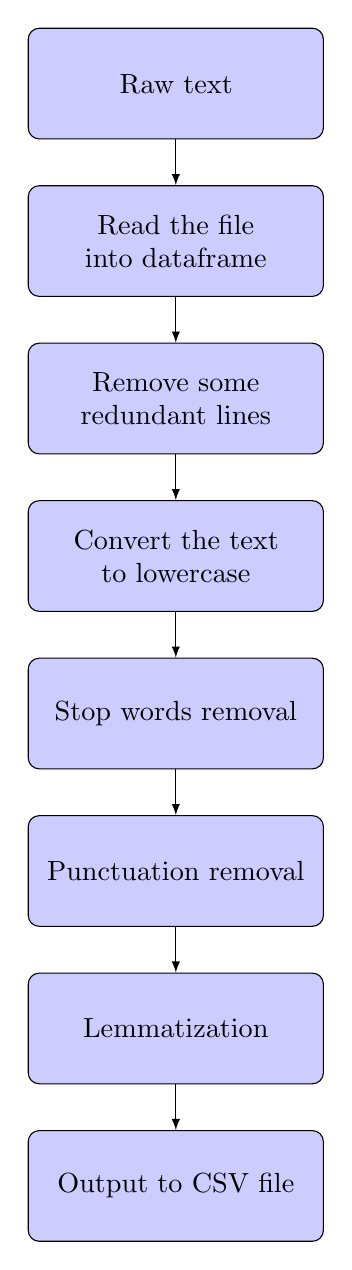
\begin{tikzpicture}[node distance = 2cm, auto]
% Place nodes
\node [block] (init) {Raw text};
\node [block, below of=init] (readDf) {Read the file into dataframe};
\node [block, below of=readDf] (lineRemoval) {Remove some redundant lines};
\node [block, below of=lineRemoval] (lower) {Convert the text to lowercase};
\node [block, below of=lower] (stopwordRemoval) {Stop words removal};
\node [block, below of=stopwordRemoval] (symRemoval) {Punctuation removal};
\node [block, below of=symRemoval] (lemmatization) {Lemmatization};
\node [block, below of=lemmatization] (output) {Output to CSV file};

% Draw edges

\path [line] (init) -- (readDf);
\path [line] (readDf) -- (lineRemoval);
\path [line] (lineRemoval) -- (lower);
\path [line] (lower) -- (stopwordRemoval);
\path [line] (stopwordRemoval) -- (symRemoval);
\path [line] (symRemoval) -- (lemmatization);
\path [line] (lemmatization) -- (output);
\end{tikzpicture}
\caption{Process flow of preprocessing the news article dataset}
\label{fig: preprocessFlow}
\end{figure}

The flow chart above illustrates the preprocessing process. The news articles dataset is in the form of raw text. Some preprocessing is needed before the features can be extracted from the text to build the text classification models. First, the raw text would be read into a dataframe or a data structure for ease of access and processing.

There are some lines in the raw text files that are irrelevant to text classification, these lines would be removed to reduce the noise in the dataset. All the text in the dataset would be converted to lowercase for uniformity and ease of processing. There are some words in the text that are useful in human speech but do not convey meanings in text analysis. These words are stop words, these words would be removed. After stop words removal, the text should contain only the words that are vital to text analysis but there would be some punctuations and symbols in the text. These punctuations and symbols would be removed as well so that the text is cleaner and contains less noise.

After that, there is an important step, lemmatization. Lemmatization would transform most of the words in the text to their root form which is known as a lemma. This would reduce the noise in the data by transforming similar words into a single word. The alternative to lemmatization would be stemming. Stemming would be faster and need less processing power than lemmatization but stemming has a drawback. The result of stemming may not be a real word because stemming just chop off the end of the words. On the other hand, lemmatization uses vocabulary and morphological analysis of words to remove the inflectional endings only, producing the root form of words. \cite{stemLemma}. Therefore, the output of lemmatization would be better than stemming.

The purpose of lemmatization is to reduced the number of distinct words in the document. The words, "good", "better", and "best" might appear in a news articles dataset. Without lemmatization, these words would be 3 distinct words. With lemmatization, all 3 of these words would be transformed to their root word which is "good". Therefore, by using lemmatization, the number of distinct words in the text would be reduced and the noise in the data would be minimized.

After all the words in the text file are lemmatized, the dataframe that contains the text is written to a CSV file. The training process would be able to read the CSV file easily and train the classification models with the method chosen.\\


\section{Overall Process Flow}
\begin{figure} [ht]
\centering
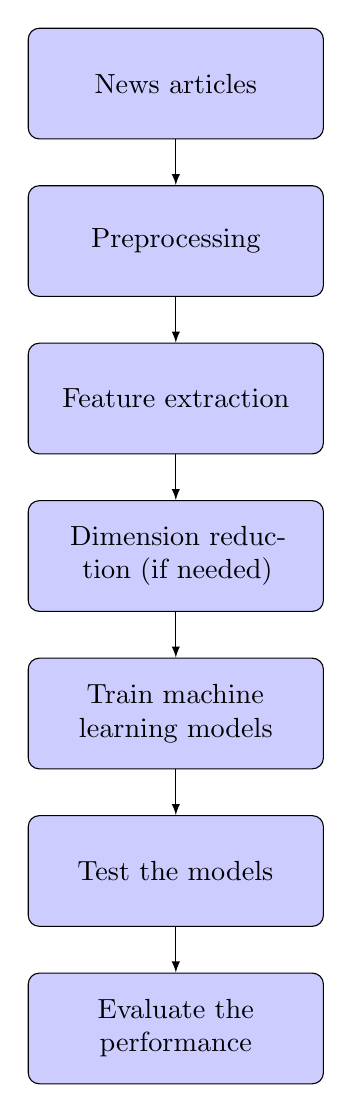
\begin{tikzpicture} [node distance = 2cm, auto]
% Place nodes
\node [block] (init) {News articles};
\node [block, below of=init] (preprocessing) {Preprocessing};
\node [block, below of=preprocessing] (feaext) {Feature extraction};
\node [block, below of=feaext] (dimred) {Dimension reduction (if needed)};
\node [block, below of=dimred] (ml) {Train machine learning models};
\node [block, below of=ml] (test) {Test the models};
\node [block, below of=test] (eval) {Evaluate the performance};
% Draw edges
\path [line] (init) -- (preprocessing);
\path [line] (preprocessing) -- (feaext);
\path [line] (feaext) -- (dimred);
\path [line] (dimred) -- (ml);
\path [line] (ml) -- (test);
\path [line] (test) -- (eval);

\end{tikzpicture}
\caption{Overall process flow}
\label{fig: overallFlow}
\end{figure}

The process flow chart above is the overall process for the few experiments. As mentioned above, the news articles dataset has to be preprocessed before it can undergo feature extraction and being used to train machine learning models.

After preprocessing, the resulting data would be used in several experiments with a few subtle differences.
The differences in the experiments would be in the feature extraction stage and the dimension reduction stage. 

There would be 2 different document representation method or feature extraction method in the experiments. An experiment would be conducted with each of the feature extraction method without dimension reduction. Several classification models would be trained with the features from both of the feature extraction methods without dimension reduction. By evaluating the performance of the classification models, a more optimized feature extraction method would be identified thus fulfilling the first objective of this study.

In a number of experiments, the feature matrix output of the 2 feature extraction method would undergo dimension reduction. There is a parameter to the dimension reduction methods to control to what extends should the feature matrix be reduced to. By manipulating this parameter, feature matrices of different dimension would be produced. These matrices with different dimension would be used as training data for classification models. Different dimension of the feature matrices would certainly has an effect on the performance of the classification models. The performance of the classification models trained with feature matrices of different dimension would be evaluated. Thus, the effect of dimension reduction has on the performance of classification models could be determined. This would fulfill the second objective of this study.

Since there are 2 document representation method and 2 dimension reduction method, there would be a combination of 4 experiments. In addition to the experiments without dimension reduction, there would be a total of 6 experiments. These experiments use different combination of document representation method, dimension reductions and all the 3 classification models. From the results of all the experiments, the best combination of document representation, dimension reduction and classification models for news articles would be identified, which is the third objective of this study.\\

\section{The dataset}
\graphicspath{{./images/}}

The dataset used in this research is the 20 news group dataset. It is freely available at \url{http://qwone.com/~jason/20Newsgroups/}. It is a collection of news articles that can be divided almost evenly to 20 groups. Some of the groups are closely related to one another and some are widely different. Categories with the same prefix for example \textit{comp} would have high similarity with one another but also subtle differences. The categories with the different prefixes, for example \textit{rec} and \textit{talk} would be very different from one another.

This characteristic of the dataset make it a good dataset to test text classification. A good classification model should be able to differentiate the different groups of news article even the groups that closely resembled one another.

The table below show the number of count for each category. There is a total of 18790 articles and most of the categories have almost 1000 articles in them. 

\begin{table} [ht]
	\centering
	\begin{tabular} {|| c | c ||}
		\hline
		Category & count \\ [0.5ex]
		\hline\hline
		alt.atheism & 798 \\
		comp.graphics & 970 \\
		comp.os.ms-windows.misc & 980 \\
		comp.sys.ibm.pc.hardware & 978 \\
		comp.sys.mac.hardware & 957 \\
		comp.windows.x & 978 \\
		misc.forsale & 962 \\
		rec.autos & 988 \\
		rec.motorcycles & 993 \\
		rec.sport.baseball & 993 \\
		rec.sport.hockey & 998 \\
		sci.crypt & 991 \\
		sci.electronics & 981 \\
		sci.med & 988 \\
		sci.space & 986 \\
		soc.religion.christian & 997 \\
		talk.politics.guns & 910 \\
		talk.politics.mideast & 940 \\
		talk.politics.misc & 774 \\
		talk.religion.misc & 628 \\
		\hline
	\end{tabular}
	\caption{The count of each category in the dataset}
	\label{tbl:freqCount}
\end{table}


The bar chart below visualized the data displayed on the table for ease of viewing. Most of categories have almost 1000 articles except alt.atheism, talk.politics.misc and talk.religion.misc.

\begin{figure} [ht]
	\centering
	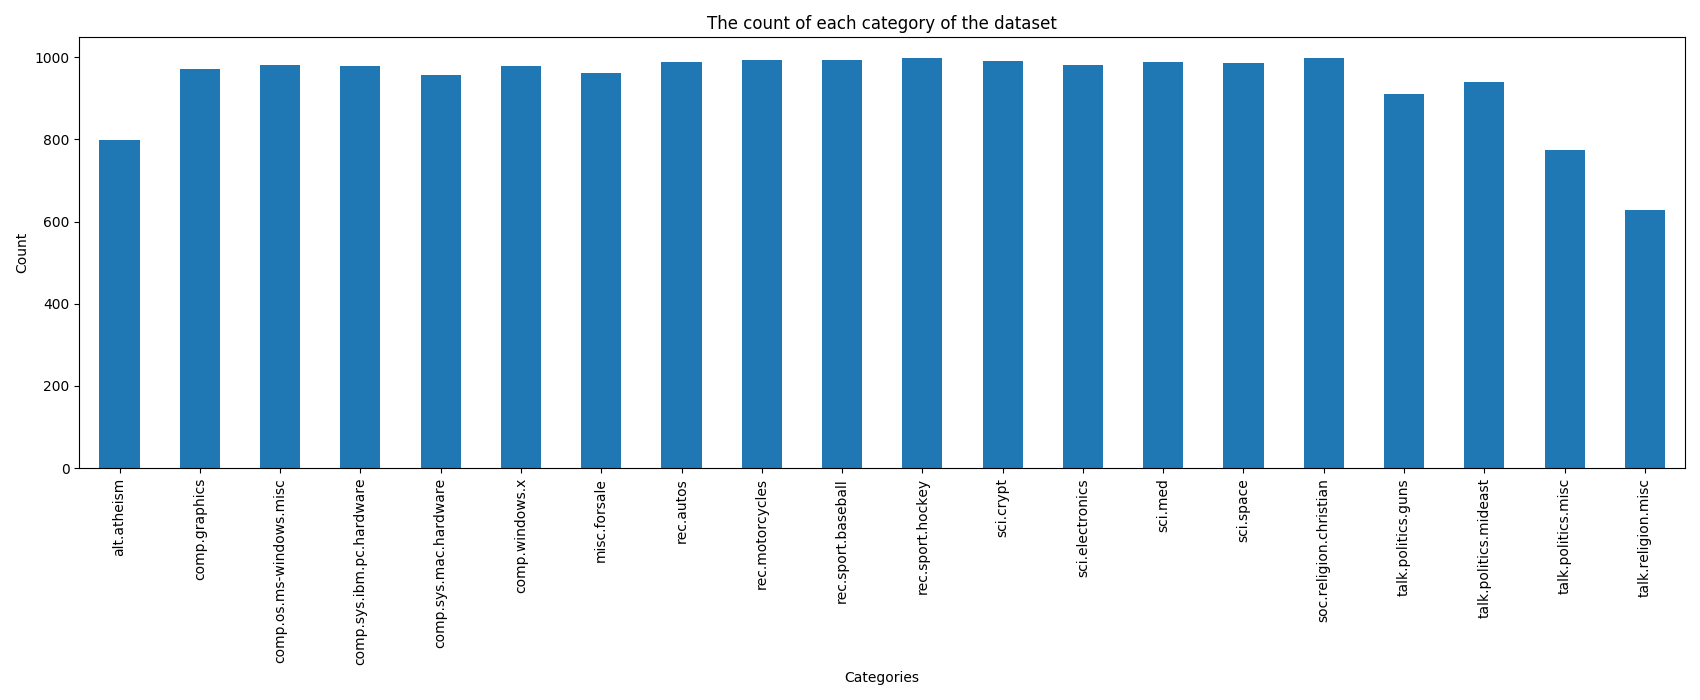
\includegraphics[width=\textwidth]{count}
	\caption{The count of each category in the dataset}
	\label{fig:freqCount}
\end{figure}

As mentioned there are 18790 articles in the data, the articles would be split at random into 8:2 ratio. 80\% of the data would be used as training data to train the classification model while 20\% of the data would be use as the test data. The training data would consist of 15032 articles while the test data would consist of 3758 articles.\\


\section{The experiments}
The experiments that has been conducted in this research is as follows:
\begin{enumerate}
	\item Term frequency
	\item Term frequency with naive dimension reduction
	\item Term frequency with truncated SVD
	\item TF-IDF
	\item TF-IDF with naive dimension reduction
	\item TF-IDF with truncated SVD
\end{enumerate}

Basically, there are 2 feature extraction method used in the experiments, namely term frequency and term frequency - inverse document frequency (\ac{tfidf}). Each of the feature extraction method would be tested with and without dimension reduction algorithm.

There are 2 dimension reduction algorithms involved, one is a naive method, which means that the features or columns lesser than a certain value would be removed. In other words, words or terms that do not appear much in the dataset would be removed. Another dimension reduction algorithm is truncated single value decomposition (\ac{svd}). This method would retain the essence of the data, the part of the data with maximum variance. 

After feature extraction and dimension reduction (if needed) are applied, the resulting features would be used to train text classification models. There are 3 text classification algorithms chosen in these experiments namely k-nearest neighbour (\ac{knn}), support vector machine (\ac{svm}), and neural network (\ac{nn}). All 3 of the machine algorithms would be applied to all the different resulting features and the accuracy scores would be evaluated.\\


\section{Conclusion}
With the method mentioned above, the experiments would be carry out and the results would be recorded. The results would be compared and the differences would be analysed.
%!TEX ROOT = main.tex

\chapter{Results and Discussions}

\section{Introduction}
The results of the experiments are shown in this section. The differences in the accuracy and performance of each of the methods would be discussed and analysed. Hopefully, the results and discussions would be able to answer the research questions posted in the beginning of this research.\\

\section{Term Frequency}

\begin{table}[H]
	\centering
	\caption{Term frequency}
	\label{tbl:termFrequency}
	\begin{tabular}{|| c | c | c | c||}
		\hline
		ML & no of features & accuracy & time taken (s) \\ [0.5ex]
		\hline\hline
		kNN & 8000 & 0.31 & 3.74 \\ 
		\hline
		SVM & 8000 & 0.81 & 5.27 \\
		\hline
		NN & 8000 & 0.84 & 91.82 \\
		\hline
	\end{tabular}
\end{table}

Term frequency is one of most common feature extraction method in text. It convert all the words in the dataset into a matrix where each column is a word and the value in each of the cells are the number of times each word appear in the text. Each row in the matrix is a document. This vector space model representation of the words would result in a sparse matrix since each of the documents only contains a subset of all the words in the whole dataset. 

In this experiment, the number of features of vector space model from term frequency extraction is limited to 8000, this is because of the memory constraint of the machine, if it is unlimited, the resulting matrix would be of bigger size and would have the risk of running out of memory while processing the matrix. 

In the results shown above, \ac{nn} achieved an accuracy of 0.84 which is the best accuracy out of the 3 classification algorithms but it is also the one that takes the longest to process which is 91.82s. \Ac{knn} took the least time to process, 3.74s but has the lowest accuracy score, 0.31. Overall performance, \ac{svm} is the best, it only took 5s to process, which is 80s less than \ac{nn} and has an accuracy of 0.81 which is comparable with \ac{nn}. 

\Ac{knn} accuracy is low in this scenario is possibly due to the sparsity of the feature matrix or vector space model. The data points are few and far in between. \Ac{knn} is designed for low dimensional data therefore it doesn't perform well in large and sparse data. The underlying reason would be due to \ac{knn} classify a new data point based on the distance of the new data point with the nearby data points. Since the other data points are few and sparse, the classification of the new data points would be biased to the few data points that are near. This bias would reduce the accuracy of the classification. \cite{knnDrawback}.

Neural Network (\ac{nn}) took the longest time to process the features, this is due to the number of hidden layers in \ac{nn}. The vector space model even though sparse has high dimension, \ac{nn} would need as much if not more neurons as the number of features to process the data. This processing would takes both time and computing power.

\Ac{svm} depends on the prominent features of the dataset, the support vectors to classify the dataset so it is relatively faster and as accurate.\\

\section{Term Frequency with Naive Dimension Reduction}

\begin{table} [h]
	\centering
	\caption{Term frequency with naive dimension reduction}
	\label{tbl:termFrequencyNaive}
	\begin{tabular}{|| c | c | c | c ||}
		\hline
		ML & no of features & accuracy & time taken (s) \\ [0.5ex]
		\hline\hline
		kNN & 6026 & 0.25 & 4.16 \\ 
		\hline
		kNN & 4058 & 0.26 & 4.22 \\ 
		\hline
		kNN & 2020 & 0.27 & 4.52 \\ 
		\hline
		kNN & 1030 & 0.30 & 5.08 \\ 
		\hline
		kNN & 508 & 0.32 & 5.14 \\ 
		\hline
		kNN & 108 & 0.30 & 5.10 \\ 
		\hline
		kNN & 54 & 0.26 & 4.77 \\ 
		\hline\hline
		SVM & 6026 & 0.81 & 6.57 \\
		\hline
		SVM & 4058 & 0.76 & 6.63 \\
		\hline
		SVM & 2020 & 0.74 & 7.85 \\
		\hline
		SVM & 1030 & 0.68 & 9.52 \\
		\hline
		SVM & 508 & 0.64 & 20.86 \\
		\hline
		SVM & 108 & 0.42 & 37.48 \\
		\hline
		SVM & 54 & 0.31 & 39.71 \\
		\hline\hline
		NN & 6026 & 0.85 & 67.65 \\
		\hline
		NN & 4058 & 0.83 & 63.72 \\
		\hline
		NN & 2020 & 0.78 & 43.38 \\
		\hline
		NN & 1030 & 0.73 & 42.89 \\
		\hline
		NN & 508 & 0.65 & 50.37 \\
		\hline
		NN & 108 & 0.41 & 82.84 \\
		\hline
		NN & 54 & 0.34 & 82.39 \\
		\hline
	\end{tabular}
\end{table}

The feature extraction method used in this experiment is same as the experiment above but dimension reduction method is applied to the resulting matrix before training. The dimension reduction algorithm used in this experiment is a naive one which means that the columns with the least occurrence of word are removed assuming those words are unimportant and would not have much influence on the accuracy.

In this experiment, \ac{knn} still has the worst performance among the 3 which is at 0.25 with 6026 number of features. As the number of features decreases to 508, the accuracy increases slightly to 0.32. As the number of features decreases, the time taken for \ac{knn} to produce the result increases from 4.16s to 4.77s.

\Ac{svm} and \ac{nn} have the same trend in this experiment, the accuracy decreases as the number of features decreases. Accuracy of \ac{svm} decreases from 0.81 to 0.31 as the number of features decreases from 6026 to 54. The time taken by \ac{svm} increases as the amount of features decreases, it increases from 6.57s to 39.71s.

The time taken by \ac{svm} increases quite drastically when the number of features decreased. Since the dimension reduction method used is a naive dimension reduction, no high computational cost functions are involved, the reduction would not take much time. The bulk of the time taken is for \ac{svm} to classify the text. The number of features in the matrix decreases thus the sparsity of the vector space model decreases, resulting in a denser vector space model. In this case, \ac{svm} need to take into account more data points to calculate an optimum hyperplane to separate the data points into different classes. Therefore, more time is taken to compute the optimum hyperplane.

On the other hand, the accuracy of \ac{nn} decreases from 0.85 to 0.34 as the number of features decreases from 6026 to 54. However, the time taken by NN fluctuates from 67.65s to 42.29s and then to 82.39s when the amount of features decreases from 6026 to 1030 then to 54. The overall decrement in time taken is possibly due to the reduction of features, less neurons are needed to process the data and thus the speedup.

\Ac{svm} and \ac{nn} performs better when there are more features, the time taken would be relatively lesser and the accuracy would be higher than in the scenarios with lesser number of features. This show that these 2 classification algorithms are able to process features in a large and sparse vector space effectively.\\

\subsection{Graph of Term Frequency with Naive Dimension Reduction}
\begin{figure} [H]
	\centering
	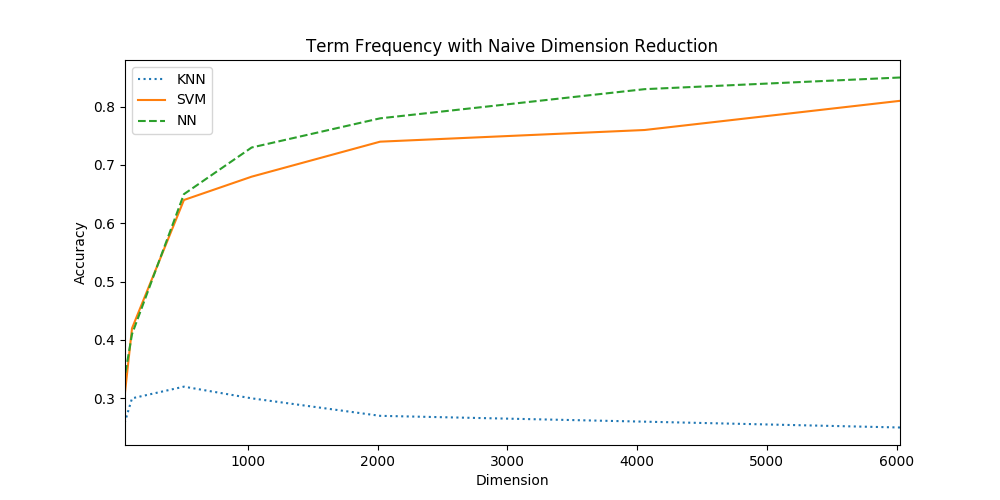
\includegraphics[width=\textwidth]{tfnaive}
	\caption{Term Frequency with Naive Dimension Reduction}
	\label{fig:tfnaive}
\end{figure}

The figure above illustrates more clearly the results shown in this section. The graph shows the change in accuracy of the classification models as the number of features decreases.

In this graph, it is clearly shown that \ac{knn} is not as efficient as \ac{svm} and \ac{nn}, its accuracy is much lower than that of \ac{svm} and \ac{nn} across the spectrum of dimension. The accuracy of \ac{knn} increases slightly as the number of features decreases.

\Ac{nn} has a slightly higher accuracy than \ac{svm} all the scenarios when the number of features is greater than 1000. When the number of features is lesser than 1000, both \ac{nn} and \ac{svm} has similar performance. The accuracy of these classification models decreases as the number of features decreases, which is expected. When the number of features decreases, the classification models would have less information to classify a document, thus the result is more error prone.\\

\section{Term Frequency with Truncated SVD}

\begin{table} [h]
	\centering
	\caption{Term frequency with truncated SVD}
	\label{tbl:termFrequencySvd}
	\begin{tabular}{|| c | c | c | c||}
		\hline
		ML & no of features & accuracy & time taken (s) \\ [0.5ex]
		\hline\hline
		kNN & 6026 & 0.29 & 809.33 \\
		\hline
		kNN & 4058 & 0.31 & 489.86 \\ 
		\hline
		kNN & 2020 & 0.39 & 222.31 \\ 
		\hline
		kNN & 1030 & 0.45 & 112.66 \\ 
		\hline
		kNN & 508 & 0.48 & 58.00 \\ 
		\hline
		kNN & 108 & 0.55 & 15.52 \\ 
		\hline
		kNN & 54 & 0.53 & 7.76 \\ 
		\hline\hline
		SVM & 6026 & 0.81 & 669.01 \\
		\hline
		SVM & 4058 & 0.79 & 391.88 \\
		\hline
		SVM & 2020 & 0.79 & 165.82 \\
		\hline
		SVM & 1030 & 0.78 & 93.1 \\
		\hline
		SVM & 508 & 0.77 & 78.48 \\
		\hline
		SVM & 108 & 0.65 & 54.03 \\
		\hline
		SVM & 54 & 0.57 & 41.11 \\
		\hline\hline
		NN & 6026 & 0.81 & 370.22 \\
		\hline
		NN & 4058 & 0.80 & 213.13 \\
		\hline
		NN & 2020 & 0.79 & 82.52 \\
		\hline
		NN & 1030 & 0.79 & 54.10 \\
		\hline
		NN & 508 & 0.77 & 35.85 \\
		\hline
		NN & 108 & 0.69 & 25.51 \\
		\hline
		NN & 54 & 0.64 & 23.01 \\
		\hline
	\end{tabular}
\end{table}

In this experiment, the feature extraction or document representation method used is still term frequency but the dimension reduction algorithm has changed. Instead of reducing the dimension of the feature matrix naively by removing the terms that has the lowest frequency, truncated \ac{svd} is used. Truncated \ac{svd} would reduce the dimension of the vector space model by retrieving the features with maximum variance in the data.

The number of features shown in the table above is the number of columns in the resulting matrix after truncated \ac{svd} is applied.

Similar with the trend in the previous experiment (term frequency with naive dimension reduction), the accuracy of \ac{knn} increases slightly, from 0.29 to 0.55 when the features decreases from 6026 to 108, but the resulting accuracy is still far from satisfactory. The time taken by \ac{knn} decreases from 809.33s to 7.76s as the number of features decreases. The trend of accuracy increment as the number of features decrease cease when the number of features is reduced to 54. \Ac{knn} accuracy decrease from 0.55 to 0.53 at that point. The fluctuation of the accuracy would be due to \ac{knn} dependency on Euclidean distance between the data points to classify a new data. As the amount of features decrease, the feature matrix becomes less sparse, \ac{knn} would need to process less data points thus the speedup. A less sparse matrix resulting from the decrement of features also make \ac{knn} classification more accurate and less biased but when the features decrease to an extent where there is no sufficient data to classify a data point correctly, the accuracy dropped.

The accuracy of \ac{svm} and \ac{nn} also have the same trend with the previous experiment, the accuracy decreases slightly when the number of features decreases. Accuracy of \ac{svm} decreases from 0.81 to 0.57 and the accuracy of \ac{nn} decreases from 0.81 to 0.64 as the number of features decreases from 6026 to 54.

As expected, the time taken by the classification model to reduce the dimension and predict the result decreases as the number of features decreases. However, when compare with previous experiments, the time taken in this experiment is astoundingly higher in the case where the features amount to 6026. \Ac{svd} would be the culprit, dimension reduction comes at a cost which is processing power. To calculate the maximum variance of the features and transform the feature matrix into a smaller dimension would require no small feats of calculation, this would consume both time and processing power.

However, the resulting accuracy is not as good as the experiment with term frequency without any dimension reduction. This is expected because the number of features decreased, the classification would have lesser information to classify a new document correctly. Therefore, it is shown that the reduction in features could reduce the memory space needed to store the feature matrix but it came at the cost of more processing power, longer processing time and most importantly a less accurate result.


Comparing the performance of the classification models in this experiment with the second experiment, term frequency with naive dimension reduction, the performance of the classification models are slightly better with \ac{svd}. All the 3 classification models has a slightly higher accuracy across the dimension size when compare with the results of the second experiment. This shows the advantage of \ac{svd} over naive dimension reduction. \Ac{svd} transformed the feature matrix into smaller dimension but retaining the maximum variance or the most prominent feature of the data. Therefore, models trained with \ac{svd} should have a better performance than those that trained with naive dimension reduction.

This experiment shows that SVD is a better dimension reduction algorithm than naive dimension reduction method. In this and the previous two experiments, term frequency is applied, it might be too simplistic and the features obtain are not optimum. The next experiments would apply a different document representation algorithm to investigate further the effect of dimension reduction has on classification model performance and compare the performance of different document representation method.\\

\subsection{Graph of Term Frequency with SVD}
\begin{figure} [H]
	\centering
	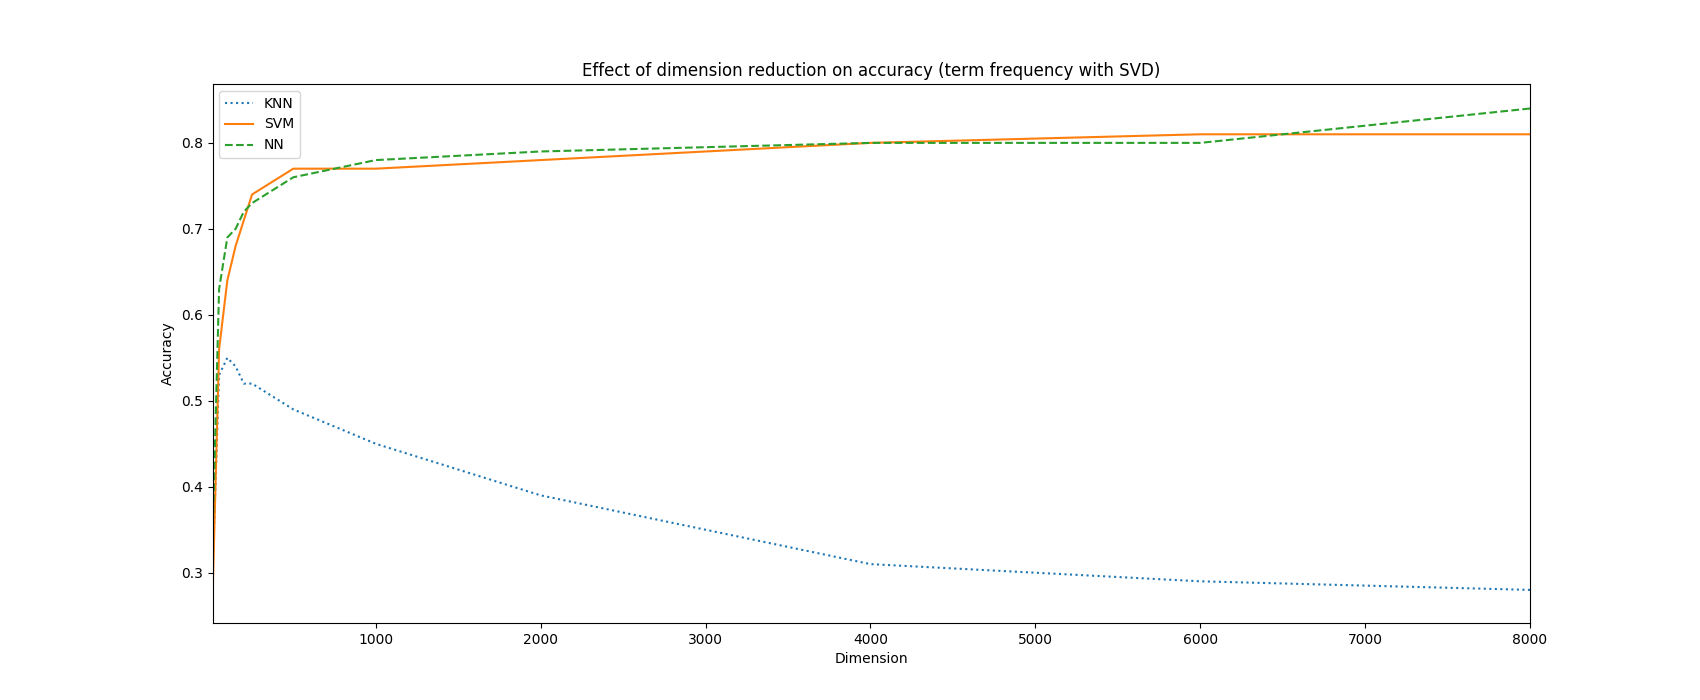
\includegraphics[width=\textwidth]{tfsvd}
	\caption{Term Frequency with SVD}
	\label{fig:tfsvd}
\end{figure}

The figure illustrates what have been described above. This graph show the advantage of SVD has over naive dimension reduction. The accuracy of \ac{knn} increases further when the dimension decreases when compare to the experiment of term frequency with naive dimension reduction. At the extreme point, \ac{knn} has an accuracy of 0.53 while in the previous experiment, \ac{knn} achieve a meager 0.26 with same number of features.

The accuracy of \ac{svm} and \ac{nn} are more stable when SVD is applied. The accuracy of both classification models does not decrease as much when the dimension decreases. Even at the extreme decrement, the accuracy achieved is better.

By comparing the result of these 2 experiments, it is seems that SVD is a better dimension reduction method. The next few experiments would explore another document representation method and determine which of the document representation methods is more efficient and optimised in extracting features from news articles.\\

\section{TF-IDF}
\begin{table} [H]
	\centering
	\caption{TF-IDF}
	\label{tbl:tfidf}
	\begin{tabular}{|| c | c | c | c||}
		\hline
		ML & no of features & accuracy & time taken (s) \\ [0.5ex]
		\hline\hline
		kNN & 8000 & 0.76 & 3.71 \\ 
		\hline
		SVM & 8000 & 0.87 & 2.39 \\
		\hline
		NN & 8000 & 0.88 & 55.82 \\
		\hline
	\end{tabular}
\end{table}

The previous experiments found that \ac{svd} has a slight edge over naive dimension reduction. In this and the next experiments, the effect on dimension reduction is further explored. The performance of the classification models in the previous experiments might be limited by the document representation method used, namely term frequency. It is a simple algorithm and the vector space model generated may not contain enough prominent features for the classification models to classify the documents accurately. Therefore, in this and the next few experiments, a different document representation method is used.
 
The document representation algorithm applied in this experiment is \ac{tfidf}. In contrast with term frequency which only take the frequency of each word into account, \ac{tfidf} takes both the frequency of each word and its rarity into account. If a term or word appear in high frequency but in many documents, this word may not be of importance and consequently is not a meaningful feature. If a word appear rarely and only in a few documents, this word would have high importance and would be a meaningful feature of the few documents.

With \ac{tfidf}, \ac{knn} can achieved a satisfactory accuracy score of 0.76 even though the number of features in the resulting matrix of \ac{tfidf} is the same with term frequency which is 8000. The vector space model of \ac{tfidf} would not be as sparse as that of term frequency which is more suitable for \ac{knn}.

\Ac{nn} is still provide the highest accuracy score of 0.88 but the time taken also the longest at 55.82s.
\Ac{nn} take the longest time to compute the result in most of the scenarios. This would be due to the number of hidden layers and the number of neurons in the \ac{nn}. In the experiments, the \ac{nn} applied has at least 1 hidden layer and the hidden layers would consist of 100 neutrons. Each of these neutron is a processing unit to compute the input feature. Due to the large size of the hidden layer and large size of the feature matrix, \ac{nn} would take a long time to feed each of the feature through the hidden layers and each of the neutron. The structure of \ac{nn} caused the long time taken, unless special hardware such as graphic processors or higher power processor is used, the time taken by \ac{nn} would be higher than other classification models.

\Ac{svm} achieved an accuracy of 0.87 which is just 0.01 shy of what achieved by \ac{nn} and the time taken is the lowest among the 3 which is 2.39s. \Ac{svm} can achieve high accuracy even with high dimension data, because \ac{svm} uses the prominent features or support vectors from the data to perform classification, \ac{svm}'s computational complexity is independent of the dimension of the data. \cite{dimRedCat}.

In comparison with the first experiment that apply term frequency document representation without dimension reduction, the performance of the classification models significantly improve. \Ac{knn} accuracy has more than doubled from 0.31 to 0.76. \Ac{svm} accuracy increases from 0.81 to 0.87 while accuracy of \ac{nn} increases from  0.84 to 0.88. Besides accuracy, the time taken also improved, time taken by \ac{svm} reduces from 5.27s to 2.39s while time taken by \ac{nn} reduces from 91.82s to 55.82s. All these improvements are achieved with the same number of features in the vector space, which is 8000. 

The performance of the classification models in this experiment is also better than those in the 2 experiments above with dimension reduction. However this may not be a fair comparison because the different number of features are used and dimension reductions are not applied in this experiment. Dimension reduction algorithms would be applied to the vector space model from \ac{tfidf} in the following experiments in order to have a fair comparison.

The performance increment from term frequency to \ac{tfidf} seems to prove that \ac{tfidf} is a better document representation method and more optimised to extract features from news articles.\\

\section{TF-IDF with Naive Dimension Reduction}

\begin{table} [ht]
	\centering
	\caption{TF-IDF with naive dimension reduction}
	\label{tbl:tfidfNaive}
	\begin{tabular}{|| c | c | c | c||}
		\hline
		ML & no of features & accuracy & time taken (s) \\ [0.5ex]
		\hline\hline
		kNN & 6026 & 0.76 & 3.76 \\ 
		\hline
		kNN & 4058 & 0.74 & 3.89 \\ 
		\hline
		kNN & 2020 & 0.69 & 4.00 \\ 
		\hline
		kNN & 1030 & 0.59 & 4.35 \\ 
		\hline
		kNN & 508 & 0.49 & 4.98 \\ 
		\hline
		kNN & 108 & 0.08 & 12.28 \\ 
		\hline
		kNN & 54 & 0.06 & 21.20 \\ 
		\hline\hline
		SVM & 6026 & 0.87 & 2.49 \\
		\hline
		SVM & 4058 & 0.85 & 2.45 \\
		\hline
		SVM & 2020 & 0.82 & 2.50 \\
		\hline
		SVM & 1030 & 0.75 & 2.64 \\
		\hline
		SVM & 508 & 0.68 & 2.98 \\
		\hline
		SVM & 108 & 0.41 & 4.43 \\
		\hline
		SVM & 54 & 0.32 & 11.63 \\
		\hline\hline
		NN & 6026 & 0.87 & 48.32 \\
		\hline
		NN & 4058 & 0.85 & 42.75 \\
		\hline
		NN & 2020 & 0.81 & 37.77 \\
		\hline
		NN & 1030 & 0.74 & 48.2 \\
		\hline
		NN & 508 & 0.65 & 80.45 \\
		\hline
		NN & 108 & 0.45 & 76.17 \\
		\hline
		NN & 54 & 0.35 & 73.92 \\
		\hline
	\end{tabular}
\end{table}

Similar with the experiment with term frequency, naive dimension reduction is applied to the vector space model generated from \ac{tfidf}. The trend over all the 3 machine learning models when the number of features decreases are similar. The accuracy of the classification models decreases and the time taken increases. 

The accuracy achieved by \ac{knn} with \ac{tfidf} plus naive dimension reduction is still passable at 0.76 when the features reduced from 8000 to 6026. \Ac{knn}'s accuracy dropped slightly to 0.69 when the number of features decreases to 20200. When the number of features decreases from 2020 to 54, the accuracy of \ac{knn} dropped for quite a large margin, from 0.69 to 0.06. The time taken by \ac{knn} increases from 3.76s to 21.20s as the features decreases.

\Ac{svm} has the same behaviour with \ac{knn} in this experiment, its accuracy decreases from 0.87 to 0.75 and then to 0.32 when the number of features decreases from 6026 to 1030 to 54. The time taken increases from 2.49s to 11.63s as the number of features decreases.

\Ac{nn} also has the similar trend in accuracy as the number of features decreases. \Ac{nn}'s accuracy decreases from 0.87 to 0.74 when the number of features decreases from 6026 to 1030. The time taken increases from 48.32s to 73.92s.

In the scenarios where the number of features are almost halved, from 8000 to 4058, the performance of the classification models are still comparable with the performance achieved with just \ac{tfidf} without any dimension reduction. The accuracy are almost the same, the time taken is similar except \ac{nn} which has quite a speedup when the number of features is reduced to 4058. This might a sweet spot between dimension reduction and accuracy. At this point, the accuracy is still satisfactory and the time taken is lesser. If \ac{nn} and dimension reduction is applied in the real world, the dimension of the news articles would have to be at this level. At this level, the classification model is best positioned to reap the reward of dimension reduction, less memory to store the feature matrix, less time is used to compute the result and a comparable accuracy is achieved.

It can be deduced that with naive dimension reduction, the number of features and memory needed to store the vector space model is reduced. With this reduced number of features, the classification models can still achieve comparable performance at a slightly decreased capacity.

The slight reduction in performance is mainly because of the reduction in dimension. As the amount of information became lesser, less information is available to train a comprehensive model. Therefore, the accuracy of the models decrease. Even though the dimension reduction applied is a naive one and less computing intensive, it still increases the time taken compared with just with \ac{tfidf}. The more reduction is performed, the time taken would increase as well.\\

\subsection{Graph of TF-IDF with Naive Dimension Reduction}
\begin{figure} [H]
	\centering
	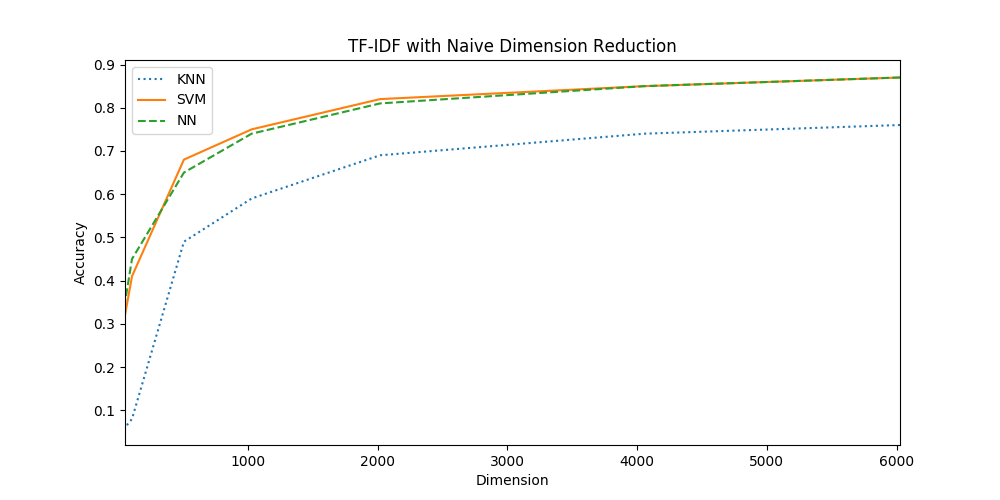
\includegraphics[width=\textwidth]{tfidfnaive}
	\caption{TFIDF with Naive Dimension Reduction}
	\label{fig:tfidfnaive}
\end{figure}

The graph above illustrates the results of this experiments. All three classification models have the same decreasing trend in their accuracy as the dimension decreases. 

\Ac{svm} and \ac{nn} have similar performance with each other. \Ac{knn} performs much better with tfidf than with term frequency document representation method but its accuracy is still lesser than that of \ac{svm} and \ac{nn}.

\section{TF-IDF with truncated SVD}

\begin{table} [h]
	\centering
	\caption{TF-IDF with truncated SVD}
	\label{tbl:tfidfSvd}
	\begin{tabular}{|| c | c | c | c||}
		\hline
		ML & no of features & accuracy & time taken (s) \\ [0.5ex]
		\hline\hline
		kNN & 6026 & 0.77 & 833.65 \\
		\hline
		kNN & 4058 & 0.77 & 487.82 \\ 
		\hline
		kNN & 2020 & 0.58 & 221.26 \\ 
		\hline
		kNN & 1030 & 0.56 & 111.36 \\
		\hline
		kNN & 508 & 0.54 & 57.40 \\ 
		\hline
		kNN & 108 & 0.69 & 15.48 \\ 
		\hline
		kNN & 54 & 0.70 & 8.04 \\ 
		\hline\hline
		SVM & 6026 & 0.87 & 374.90 \\
		\hline
		SVM & 4058 & 0.87 & 194.99 \\
		\hline
		SVM & 2020 & 0.86 & 72.16 \\
		\hline
		SVM & 1030 & 0.85 & 35.19 \\
		\hline
		SVM & 508 & 0.83 & 18.41 \\
		\hline
		SVM & 108 & 0.77 & 6.40 \\
		\hline
		SVM & 54 & 0.74 & 4.68 \\
		\hline\hline
		NN & 6026 & 0.86 & 384.91 \\
		\hline
		NN & 4058 & 0.86 & 203.26 \\
		\hline
		NN & 2020 & 0.84 & 86.47 \\
		\hline
		NN & 1030 & 0.82 & 52.29 \\
		\hline
		NN & 508 & 0.81 & 46.11 \\
		\hline
		NN & 108 & 0.79 & 27.63 \\
		\hline
		NN & 54 & 0.78 & 25.36 \\
		\hline
	\end{tabular}
\end{table}

In this last experiment, truncated \ac{svd} dimension reduction is applied to the resulting vector space model from \ac{tfidf}. Similar with experiment before, each of the classification models would be tested with several set of vector space model, each with different number of features. To put it in perspective, the number of features without reduction is 8000. 

When the number of features are at 4058 which is about halved, \ac{knn} still can produced an accuracy of 0.77 which is similar with what is achieved with \ac{tfidf} without dimension reduction. The same goes to \ac{svm} and \ac{nn}, at 4058 features, the accuracy are quite similar with \ac{tfidf} without dimension reduction. However, when the dimension of the vector space model is reduced to 2020, the accuracy across the 3 classification models dropped. \Ac{knn} being the most drastic, its accuracy dropped to 0.58 while \ac{svm} and \ac{nn} dropped to 0.86 and 0.84 respectively, which is slightly worse than before but it is still satisfactory.

Comparing with the results of the experiment with \ac{tfidf} and naive dimension reduction, this performance of the classification models with truncated \ac{svd} has a slight advantage. The accuracy is slightly better with truncated \ac{svd} than that with naive dimension reduction. This would be due to the advantage of truncated \ac{svd} obtaining the maximum variance of the features over naive dimension reduction.

The time taken in this experiment is much higher than the experiment of \ac{tfidf} without dimension reduction and \ac{tfidf} with naive dimension reduction, which is expected. This would be due to \ac{svd} reduction takes more time, as more calculations are needed to transform the data. However, the time taken decreased when further reduction is done, \ac{knn} take 833.65s to reduce the vector space model from 8000 to 6026 but just 8s to reduce the vector space model from 8000 to 54. Keep in mind that the time recorded here includes the time taken for the classification model to predict the test set as well as the dimension reduction time. This trend appear in \ac{svm} and \ac{nn} as well. \Ac{svm} took 374.90s to reduce 8000 to 6026 but just 4.64s to reduce 8000 to 54 while \ac{nn} took 384.91s to reduce 8000 to 6026 and 25.36s to reduce 8000 to 54. 

The decrement in time could be due to SVD reduced the features and only return the most prominent features of the news articles. These prominent features would make the differences between the categories of news articles more obvious to the classification models. Thus, the time taken to process the features is also reduced, a speedup. This speedup comes at a cost which is accuracy. For \ac{svm} and \ac{nn}, the reduction in accuracy is slight thus it would be logical to trade the slight accuracy with the speedup but in \ac{knn}, the trade off would be lopsided in the favour of time taken.\\

\subsection{Graph of TF-IDF with SVD}
\begin{figure} [H]
	\centering
	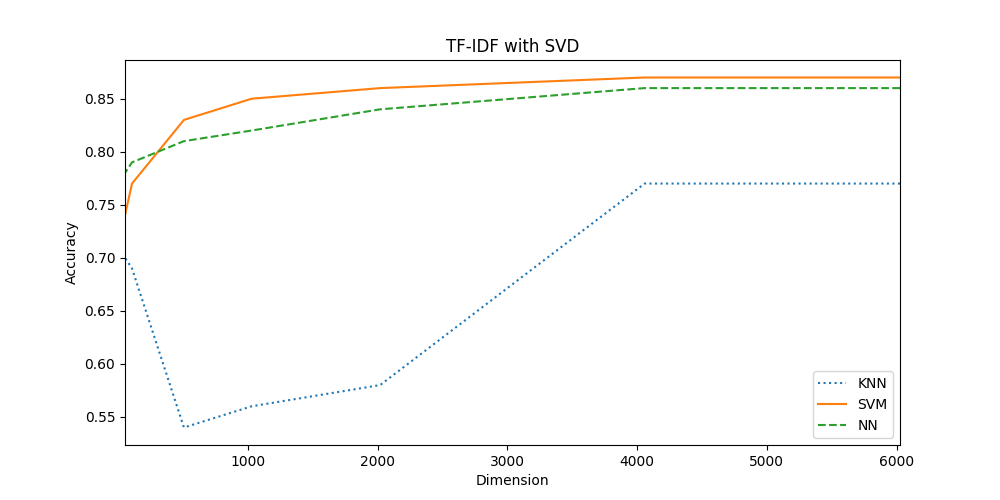
\includegraphics[width=\textwidth]{tfidfsvd}
	\caption{TFIDF with SVD}
	\label{fig:tfidfSVD}
\end{figure}

This figure show the fluctuations of the accuracy of the classification models as the dimension decreases. The feature extraction method used here is \ac{tfidf} and the dimension reduction algorithm used is truncated \ac{svd}.

\Ac{knn} accuracy remain stable at around 0.77 as the dimension decrease from 8000 to around 4000. After 4000, further decrement in dimension resulting in a decrease in accuracy. The accuracy of \ac{knn} deflected and increase from 0.54 to 0.70 when the dimension reduce from 508 to 54.

Similar to previous result, \ac{svm} and \ac{nn} accuracy remain stable around 0.8 as the dimension reduces from 8000 to 508. When the dimension of the feature matrix is reduced to an extreme of 54 then the accuracy of both \ac{svm} and \ac{nn} deteriorated to around 0.7.

\Ac{svm} is the best classification model out of the 3, it has slightly better performance than \ac{nn} in most of the scenarios. It is most resilient to the changes in dimension. This is because \ac{svm} depend on the prominent features of the data to classify the data into different classes, the dimension of the data do not has much influence on \ac{svm} computational complexity. \cite{dimRedCat}. \Ac{nn} has comparable accuracy with \ac{svm} but it would take longer time than \ac{svm} to produce the similar result.\\


\section{Conclusion}
From the results of the 6 experiments above, it is found that \ac{tfidf} is a better document representation algorithm than term frequency. The resulting vector space model from \ac{tfidf} can achieve a higher accuracy than that of term frequency. 

The effect of dimension reduction on the accuracy of the classification models is analysed. Dimension reduction, naive and truncated \ac{svd}, do reduce the dimension of the vector space model, reducing the memory needed to store the matrix. However, this reduction in features and information would result in a loss of accuracy. truncated \ac{svd} would be the better dimension reduction algorithm compared to the naive method because the accuracy achieved with truncated \ac{svd} is higher than that of the naive method.

Among the 3 classification models tested in the experiments, \ac{svm} is the most efficient and versatile. \Ac{svm} can achieve high accuracy (> 0.80) in most scenarios. \Ac{nn} can also achieve high accuracy in most of the cases tested but \ac{nn} is more time consuming. \Ac{svm} has an advantage over \ac{nn} on the aspect of processing time. Therefore, \ac{svm} would be the most efficient text classification model among the 3 classification models.


%!TEX ROOT = main.tex
\chapter{Conclusion}
It is known that TF-IDF should be better than term frequency but in the kNN article [reference], it is mentioned that term frequency is applied with naive dimension reduction and the accuracy of the model is satisfactory. Therefore, this research compare term frequency and TF-IDF and apply dimension reduction to both.

From the results of the experiments it has been confirmed that TF-IDF is a better document representation method than term frequency. Even though, with term frequency as the document representation method, SVM and NN are able to achieve satisfactory accuracy, the accuracy achieved with TF-IDF is slightly higher. The advantage of TF-IDF is more obvious, with term frequency the accuracy is a meagre 0.31 but with TF-IDF, the accuracy is 0.76 which is close to 0.80.

By applying the 2 types of dimension reduction to both the document representation method, the effect of dimension reduction on the performance of the classification models would be discovered. The classification models accuracy from both naive dimension reduction and SVD are quite similar, with SVD has a slight edge.

As the dimension of the vector space model is reduced, the accuracy of the classification models would decreased due to the lack of features or information. This reduction of features would reduce the memory used to store the vector space model. However, the reduction process would need intensive computing power and time, especially in the case of SVD.



answer the research questions and achieve the objectives of course\\

objectives:\\
1. to identify a document representation algorithm that is optimized\\
2. to investigate ML and find the most suitable\\
3. to evaluate the effect of dimension reduction has on document representation and document classification model performance\\

questions:\\
1. which dimension reduction algorithm is optimized\\
2. how complexities of the features influence the accuracy\\
3. the best ML\\

\bibliography{myrefs}

\begin{appendices}
%!TEX ROOT = main.tex
\chapter{Code}
\end{appendices}

\end{document}
